\subsection{Layers Tab}

In the 'Layers' tab, a tree view is given to configure the display of the existing elements. 

\begin{figure}[H]
  \center
    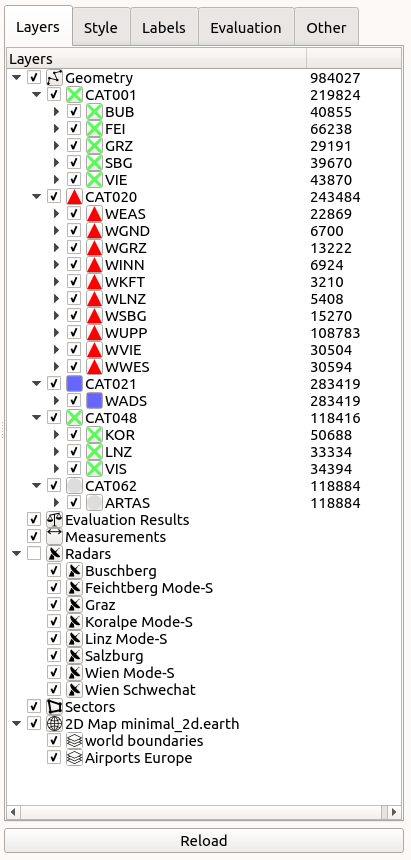
\includegraphics[width=9cm,frame]{figures/geoview_config_panel.png}
  \caption{Geographic View layers tab}
\end{figure}

The following main tree elements are:\\

\begin{itemize}
 \item Geometry: Shows currently loaded DBConent
 \item Measurements: Shows the current distance measurements
 \item Radars: Shows the existing radars 
 \item Sectors: Shows the existing sectors
 \item Map: Shows current map layers
\end{itemize} 
 \ \\

How the geometry is layered is defined by the Layer mode in the Style tab, please refer to \nameref{sec:layer_mode} for details. \\
 
\includegraphics[width=0.5cm]{../../data/icons/hint.png} For all geometry layers, a second colum is shown, giving the count of number of target reports in the (sub-) layer (as were loaded from the database). \\
 
In the Layers widget, a number of operations are possible for each tree item.

\begin{table}[H]
  \center
  \begin{tabular}{ | l | l | l |}
    \hline
    \textbf{Operation} & \textbf{Trigger} &  \textbf{Description} \\ \hline
    View sub-items & Triangle & Opens or closes view of the sub-items \\ \hline
    Display item & Checkbox & Enables or disables display of items (and all sub-items) \\ \hline
    Display context menu & Click on symbol & Opens the items context menu \\ \hline
  \end{tabular}
  \caption{Layer operations}
\end{table}

The context menu allows several actions to be performed on an item. If an item has sub-items, the same action will automatically be performed on the child items.

\subfile{geo_layers_geo_ops}

\subfile{geo_layers_measure_ops}

\subfile{geo_layers_radars_ops}

\subfile{geo_layers_sectors_ops}

\subfile{geo_layers_map_ops}
